\chapter{Исследовательская часть}

\section{Среда для тестирования}

Для тестирования разработанного алгоритма применялась облачная платформа Google Colab, не требующая установки ПО на локальный компьютер.

\section{Исследование признаков}

\begin{figure}
	\begin{center}
		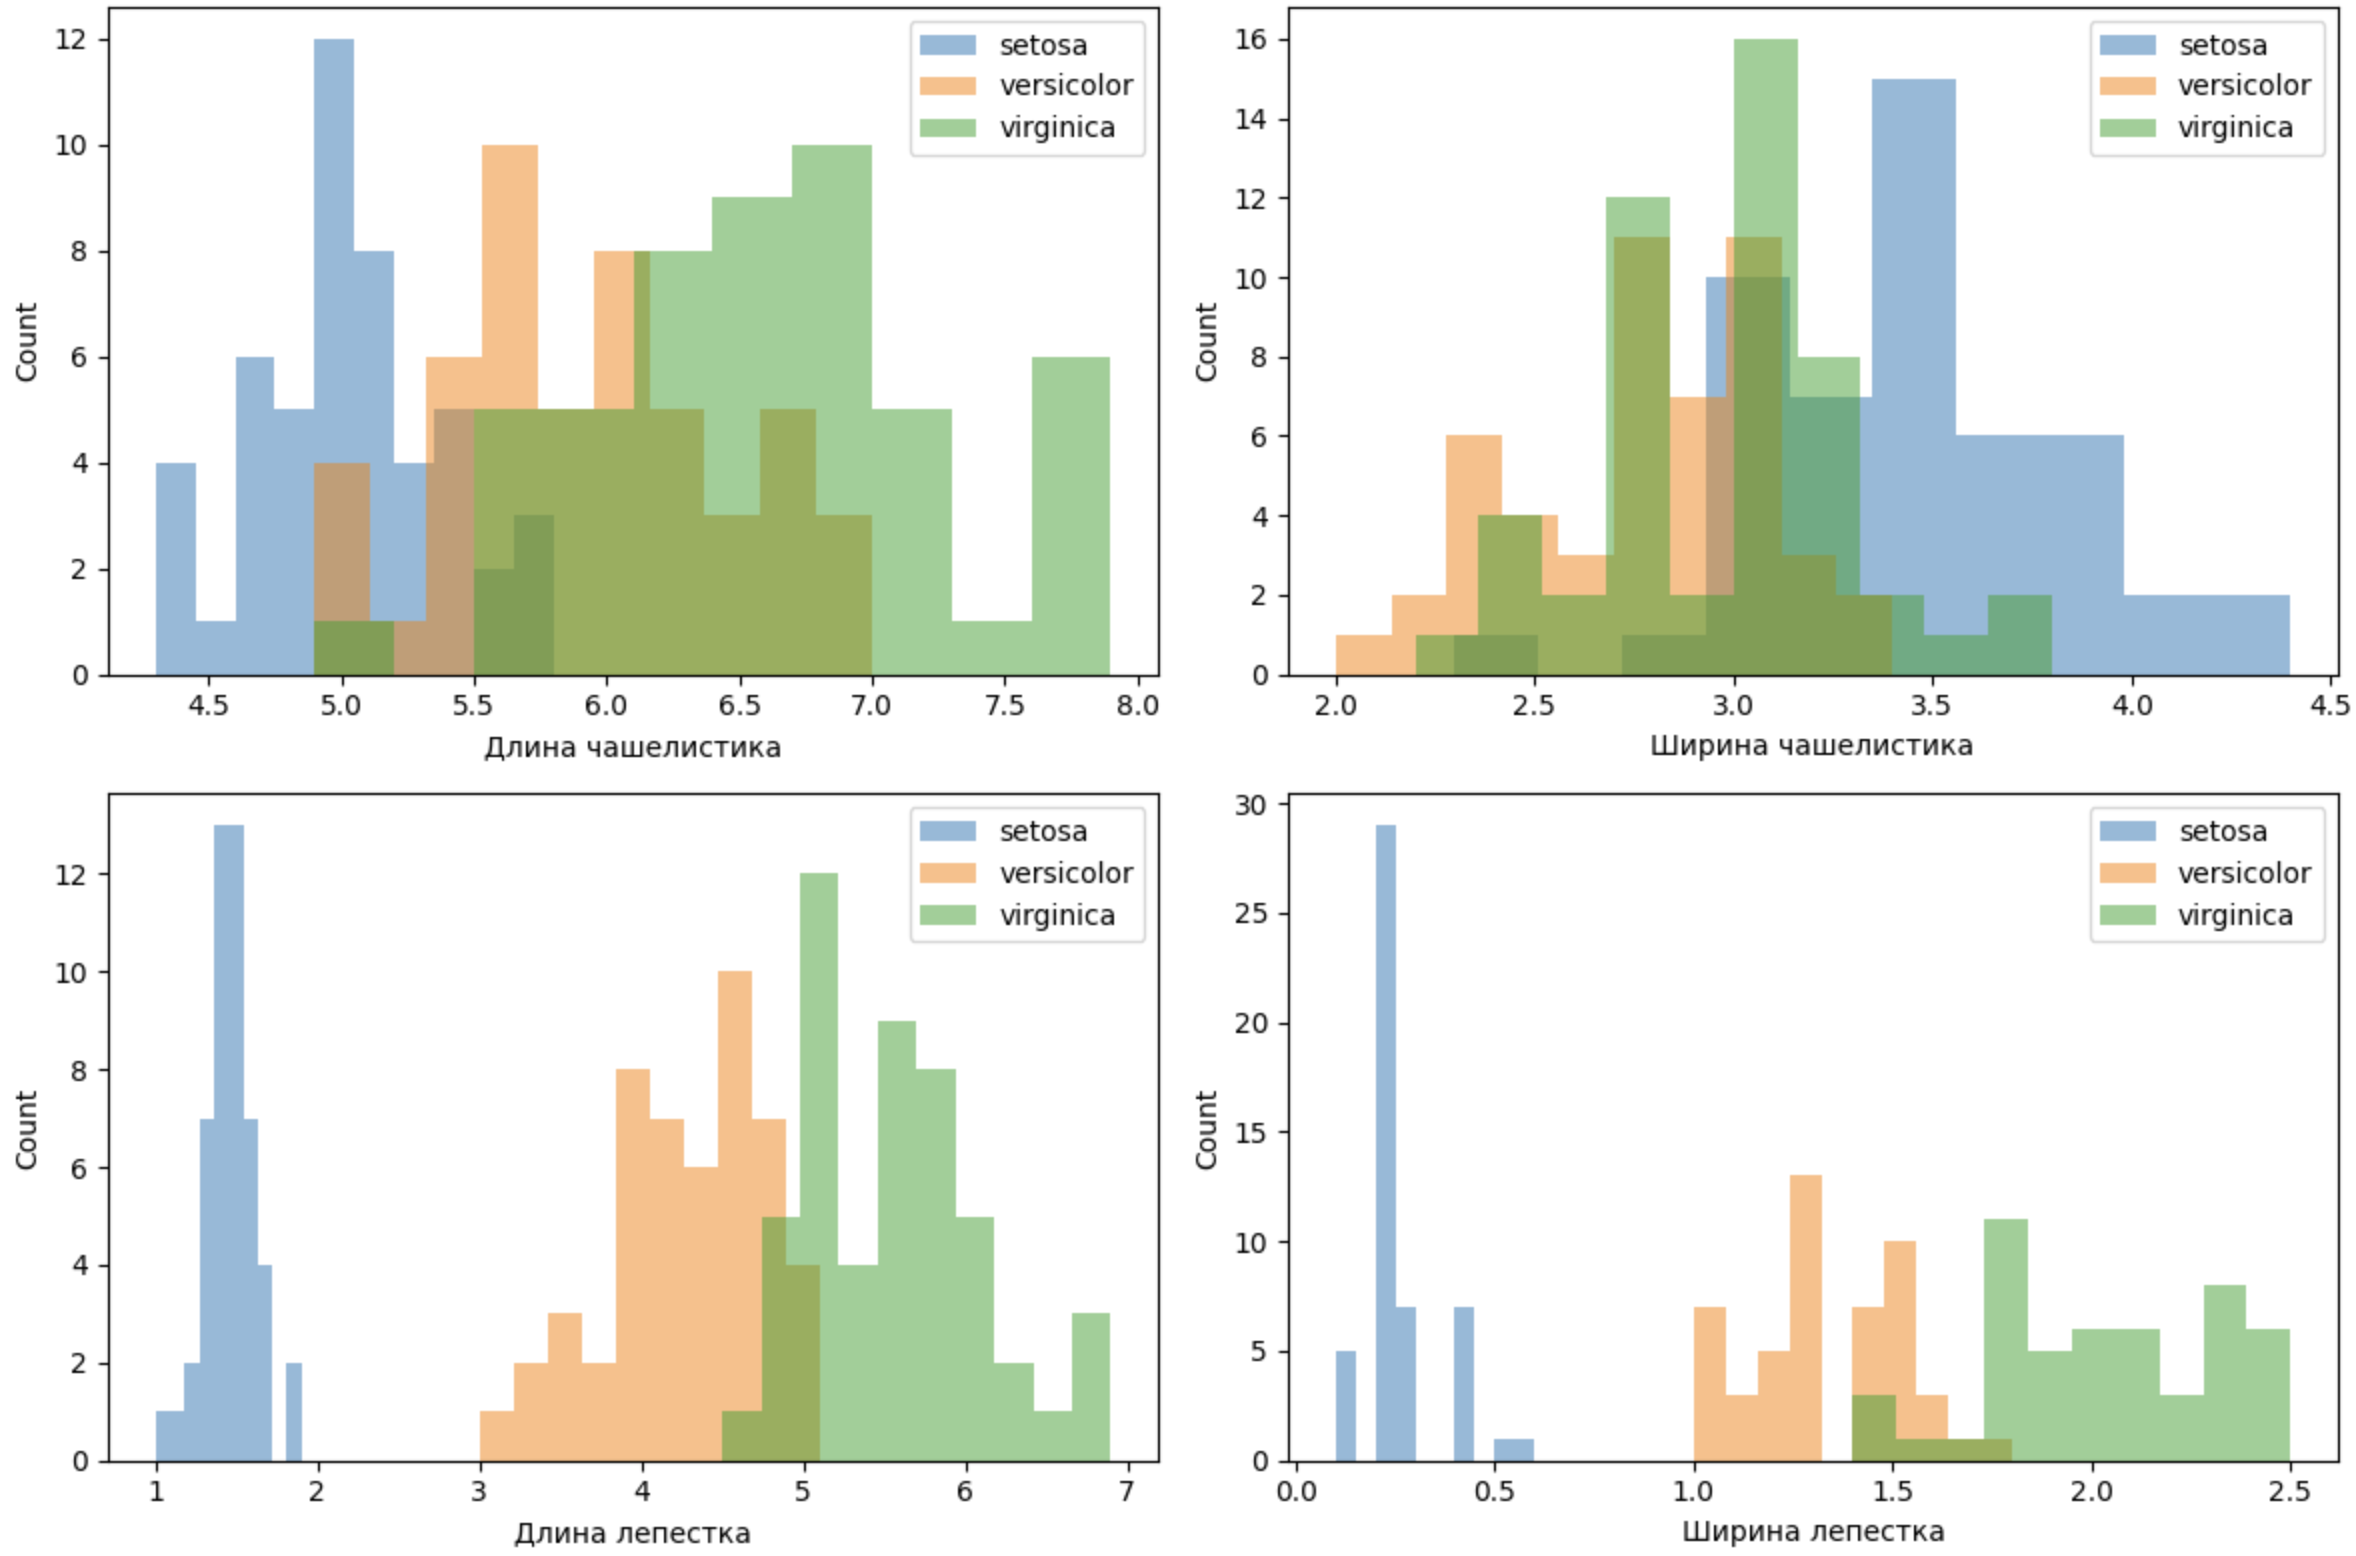
\includegraphics[width=\textwidth]{images/1.png}
	\end{center}
	\caption{Гистограммы распределения значений для каждого признака и для каждого класса}
	\label{img:1}
\end{figure}

\begin{figure}
	\begin{center}
		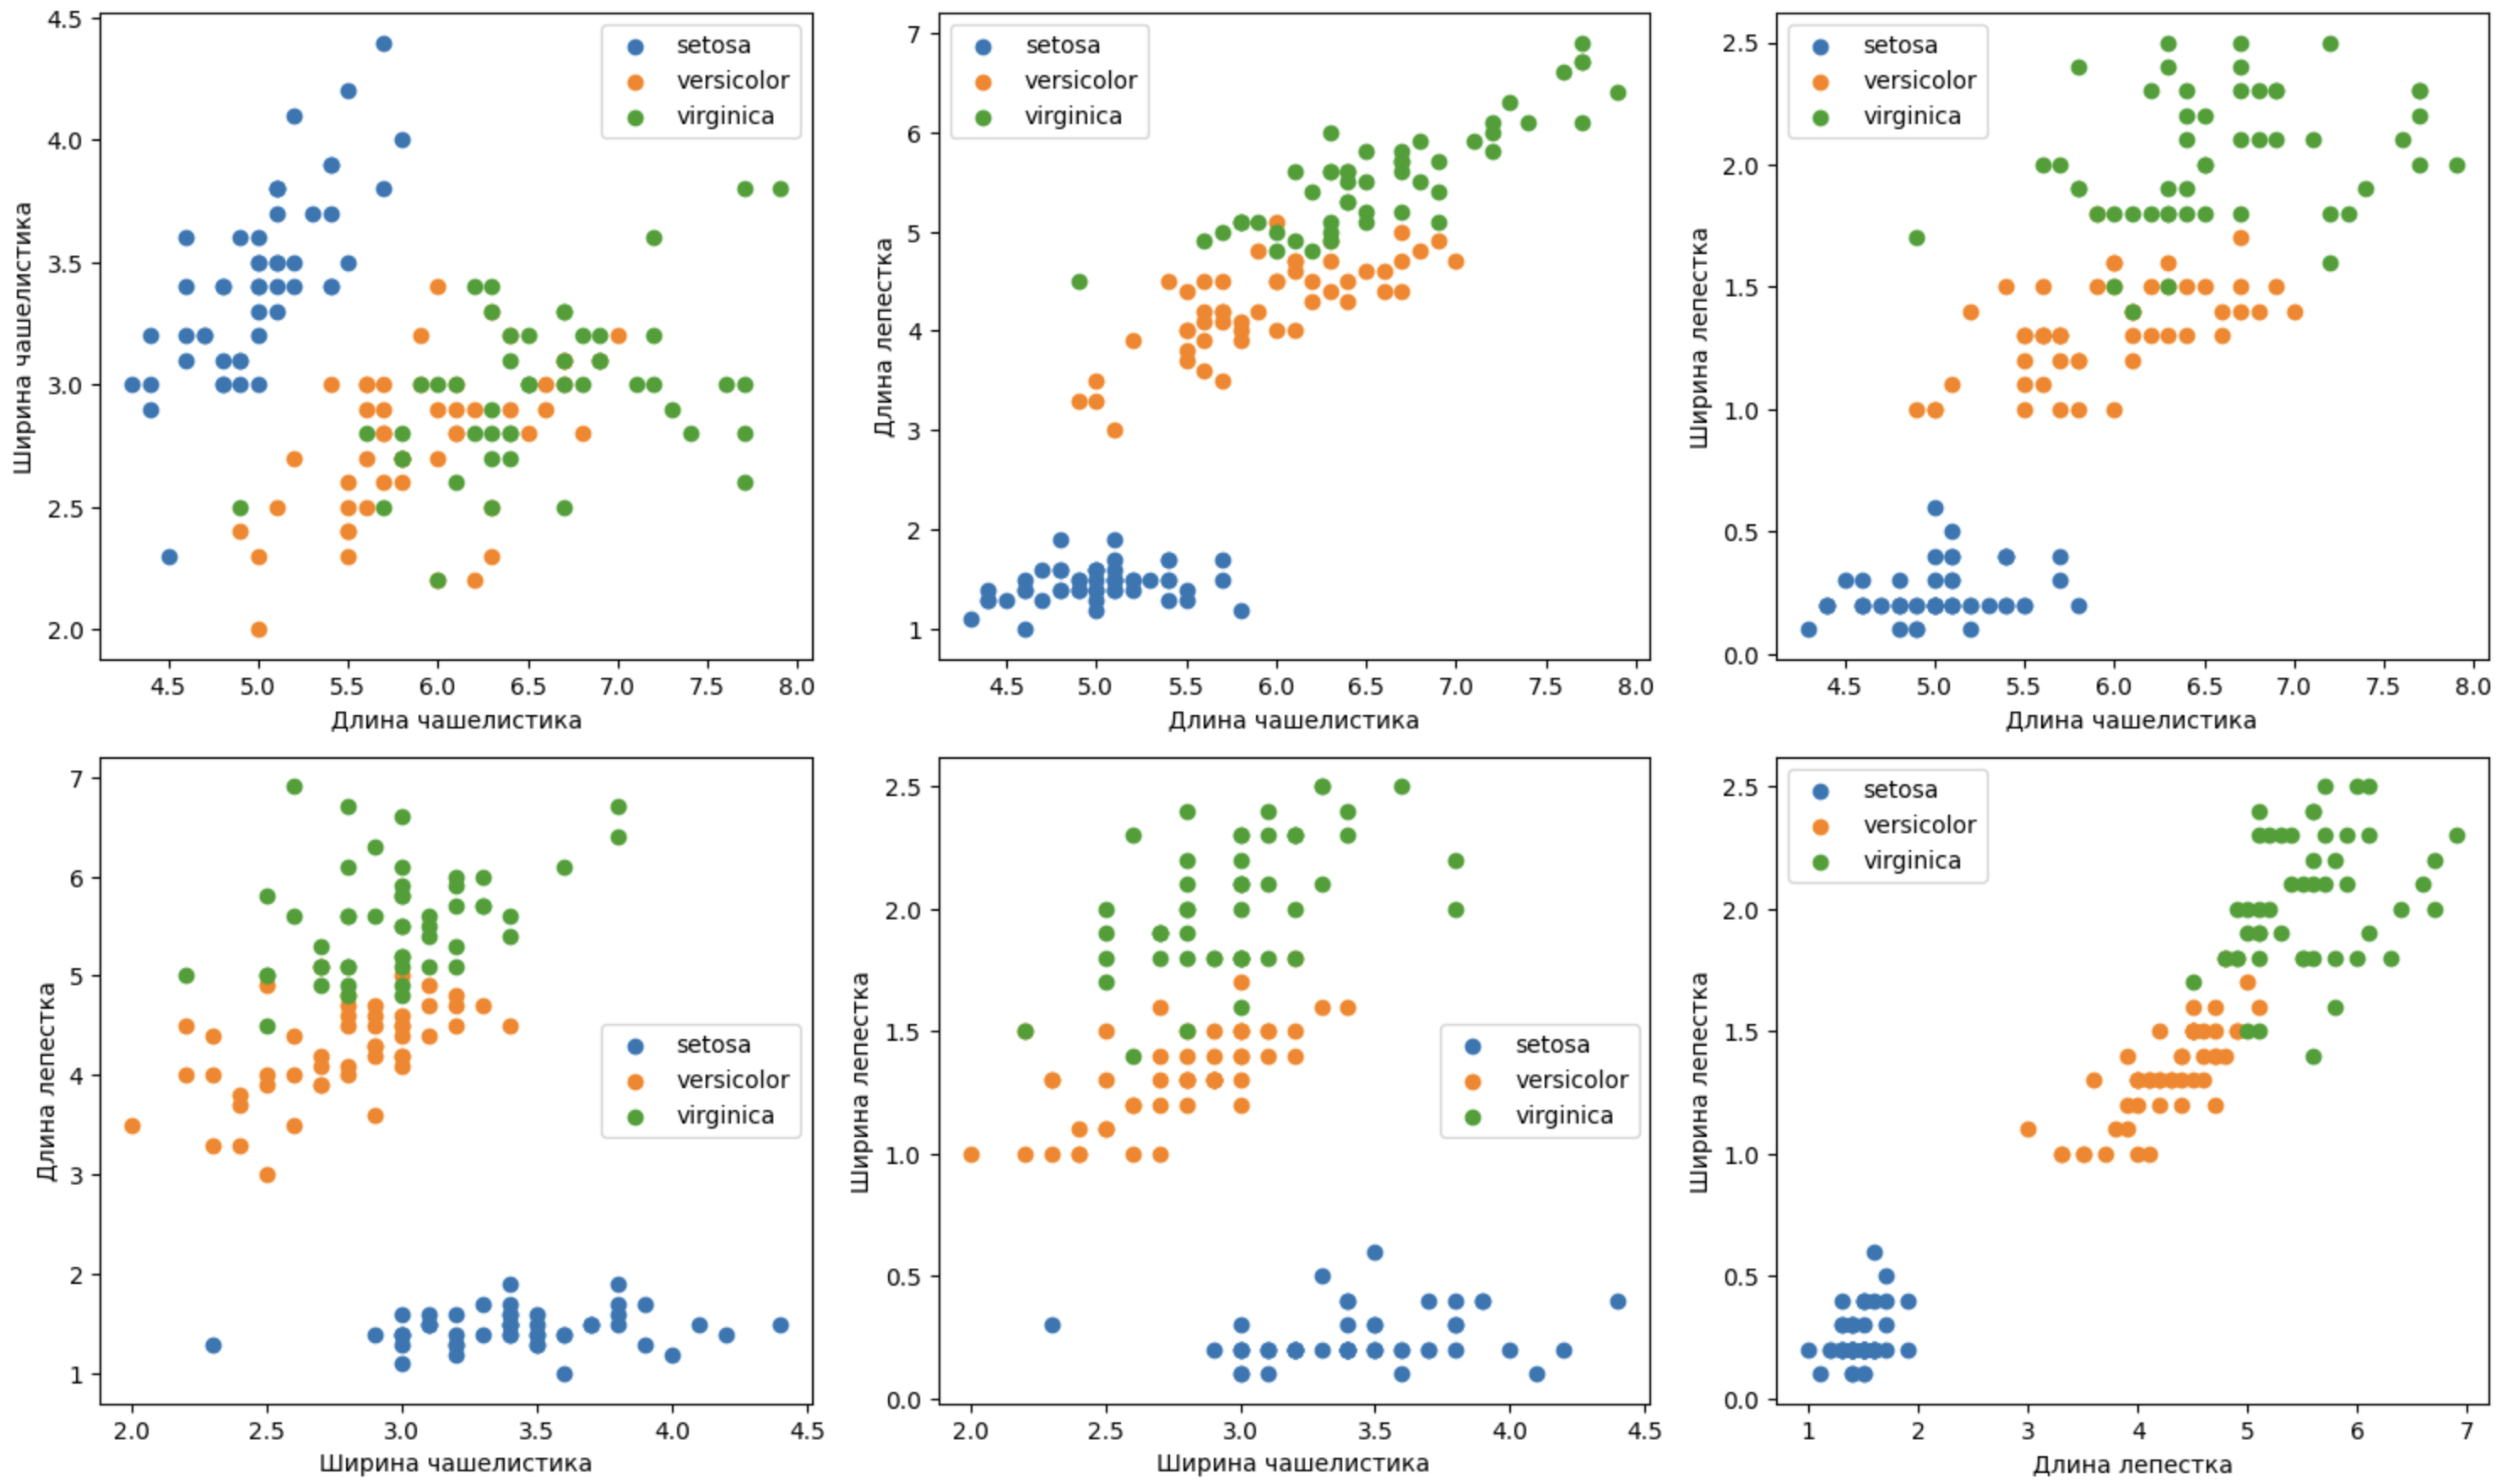
\includegraphics[width=\textwidth]{images/2.png}
	\end{center}
	\caption{Визуализация проекций классов на все возможные пары признаков}
	\label{img:2}
\end{figure}

\begin{figure}
	\begin{center}
		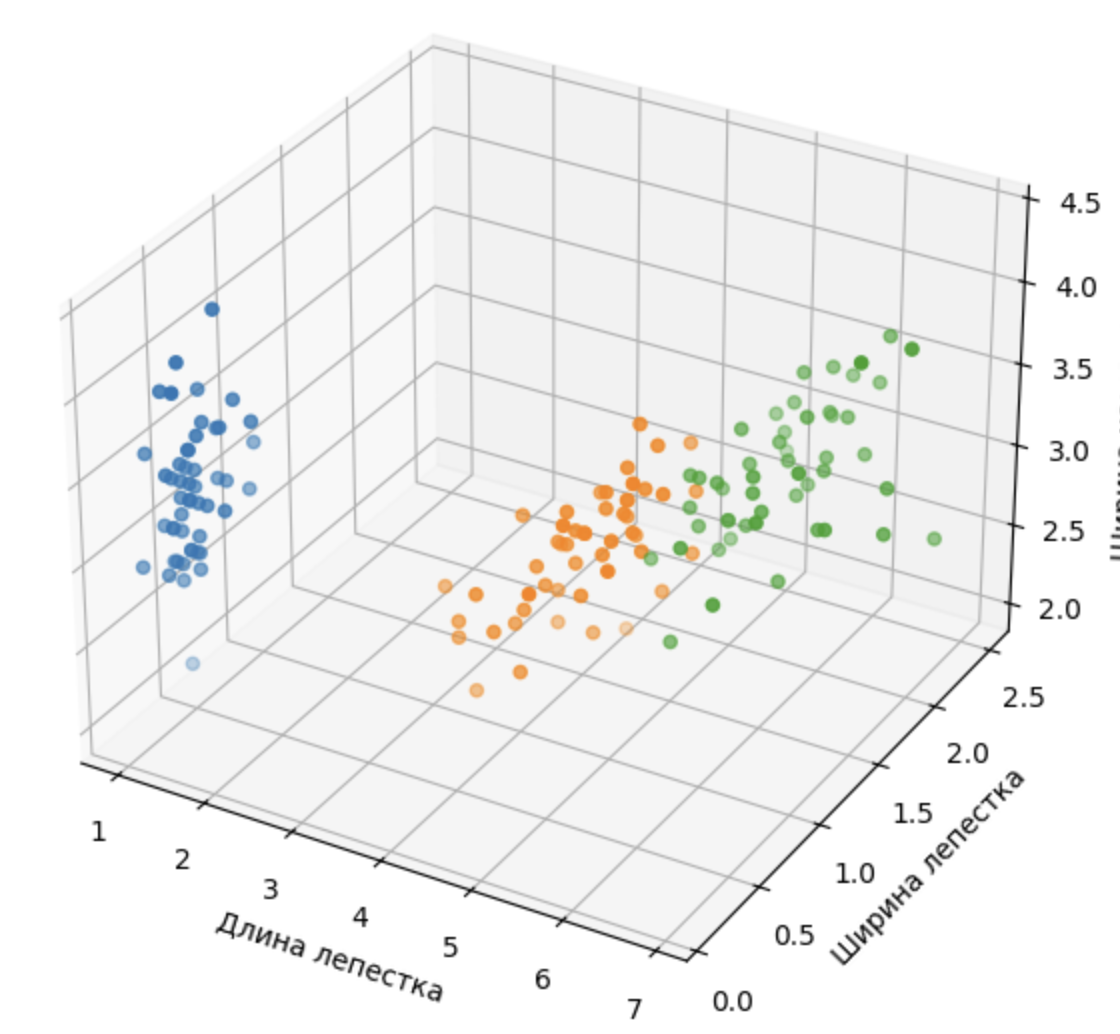
\includegraphics[width=\textwidth]{images/3.png}
	\end{center}
	\caption{Визуализация проекций классов на пространство признаков {<<Длина лепестка>>, <<Ширина лепестка>>, <<Ширина чашелистника>>}}
	\label{img:3}
\end{figure}

\begin{figure}
	\begin{center}
		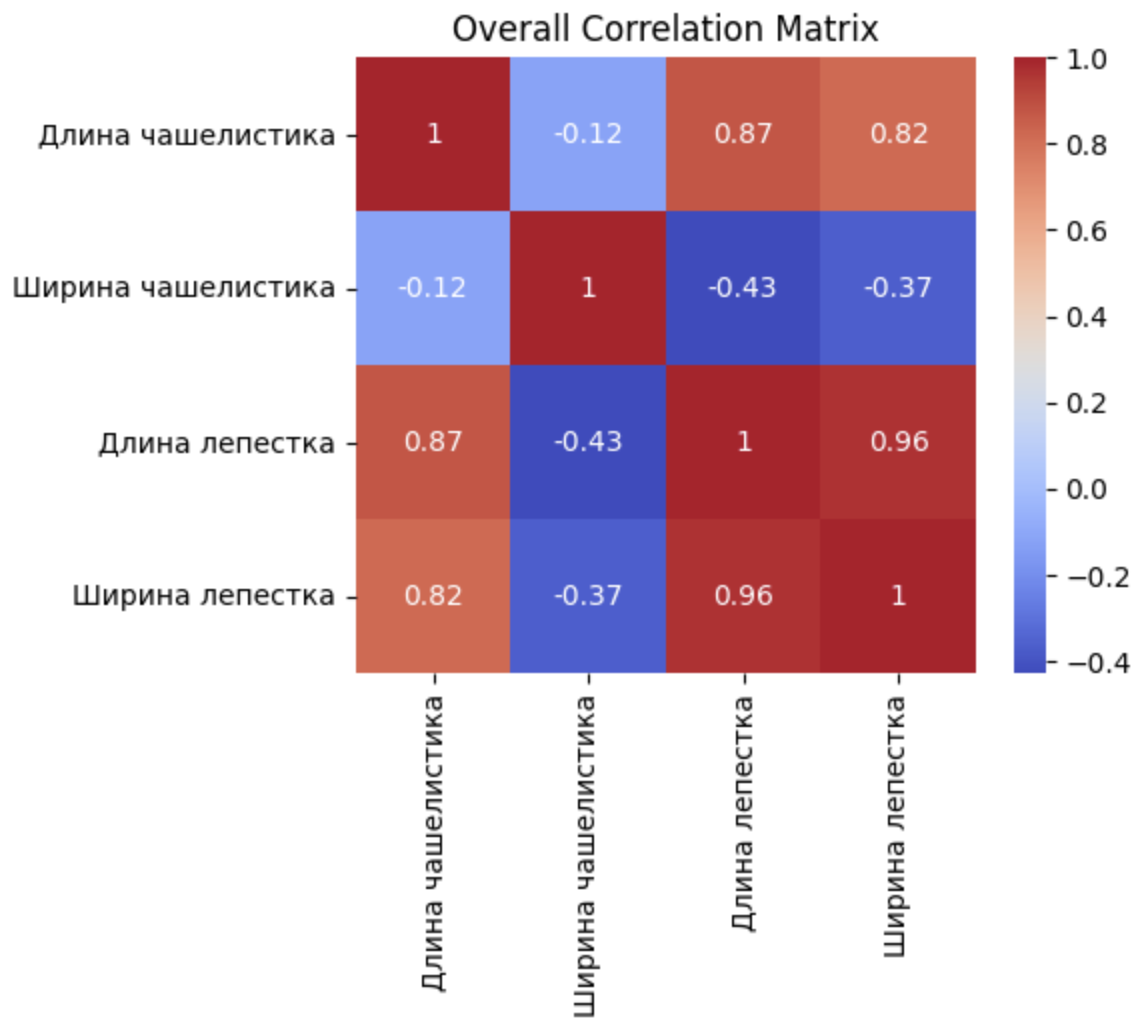
\includegraphics[width=\textwidth]{images/4.png}
	\end{center}
	\caption{Матрица корреляции признаков по всем классам}
	\label{img:4}
\end{figure}

\begin{figure}
	\begin{center}
		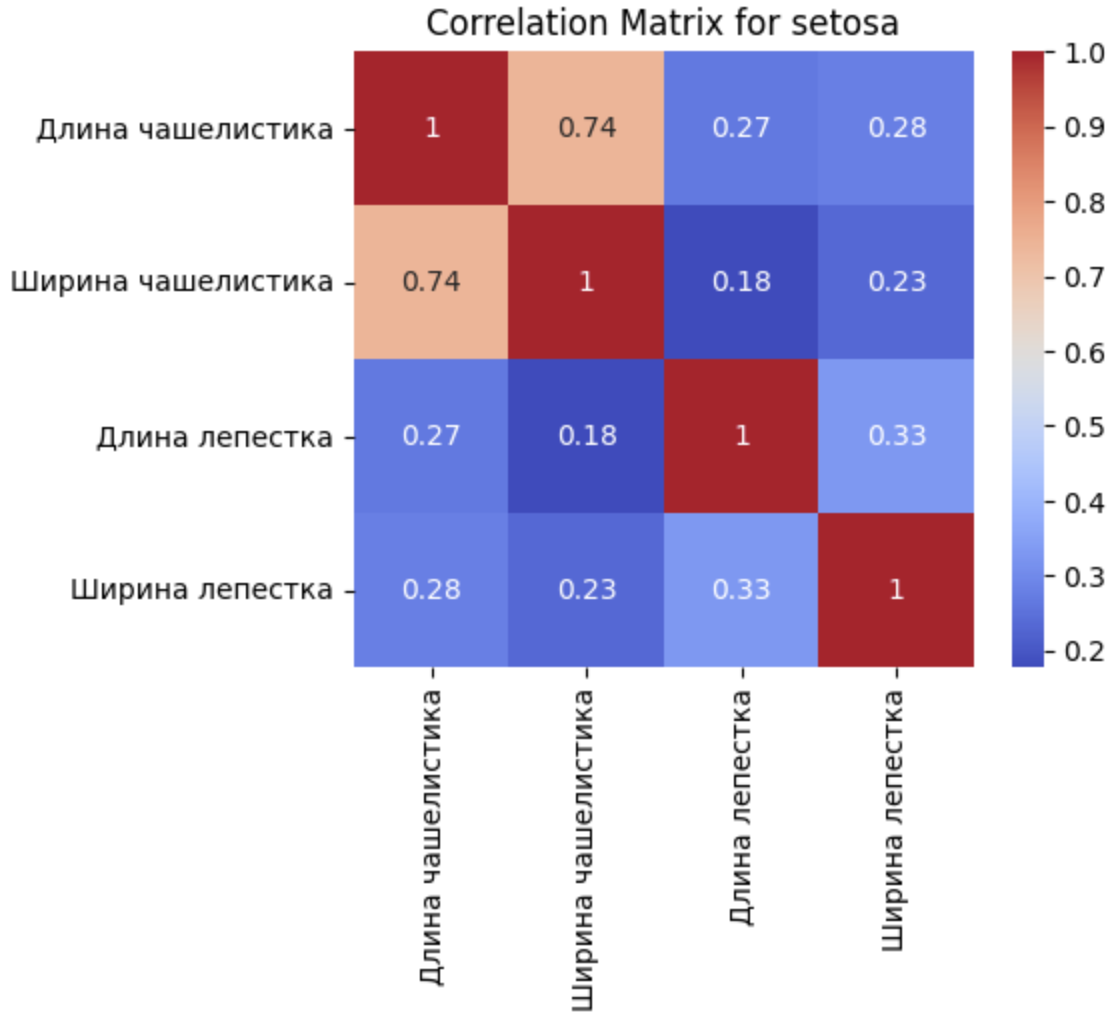
\includegraphics[width=\textwidth]{images/5.png}
	\end{center}
	\caption{Матрица корреляции признаков для класса <<setosa>>}
	\label{img:5}
\end{figure}

\begin{figure}
	\begin{center}
		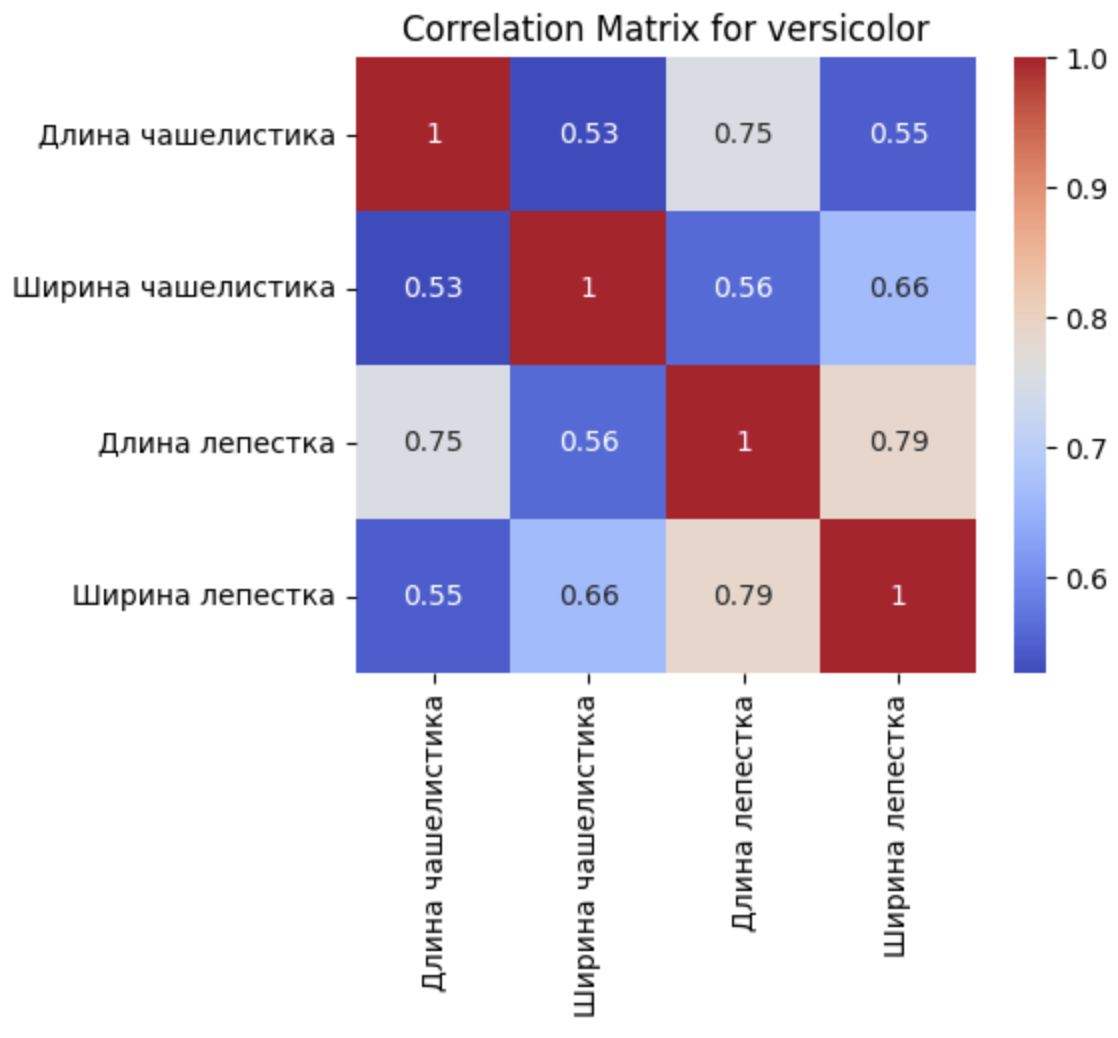
\includegraphics[width=\textwidth]{images/6.png}
	\end{center}
	\caption{Матрица корреляции признаков для класса <<versicolor>>}
	\label{img:6}
\end{figure}

\begin{figure}
	\begin{center}
		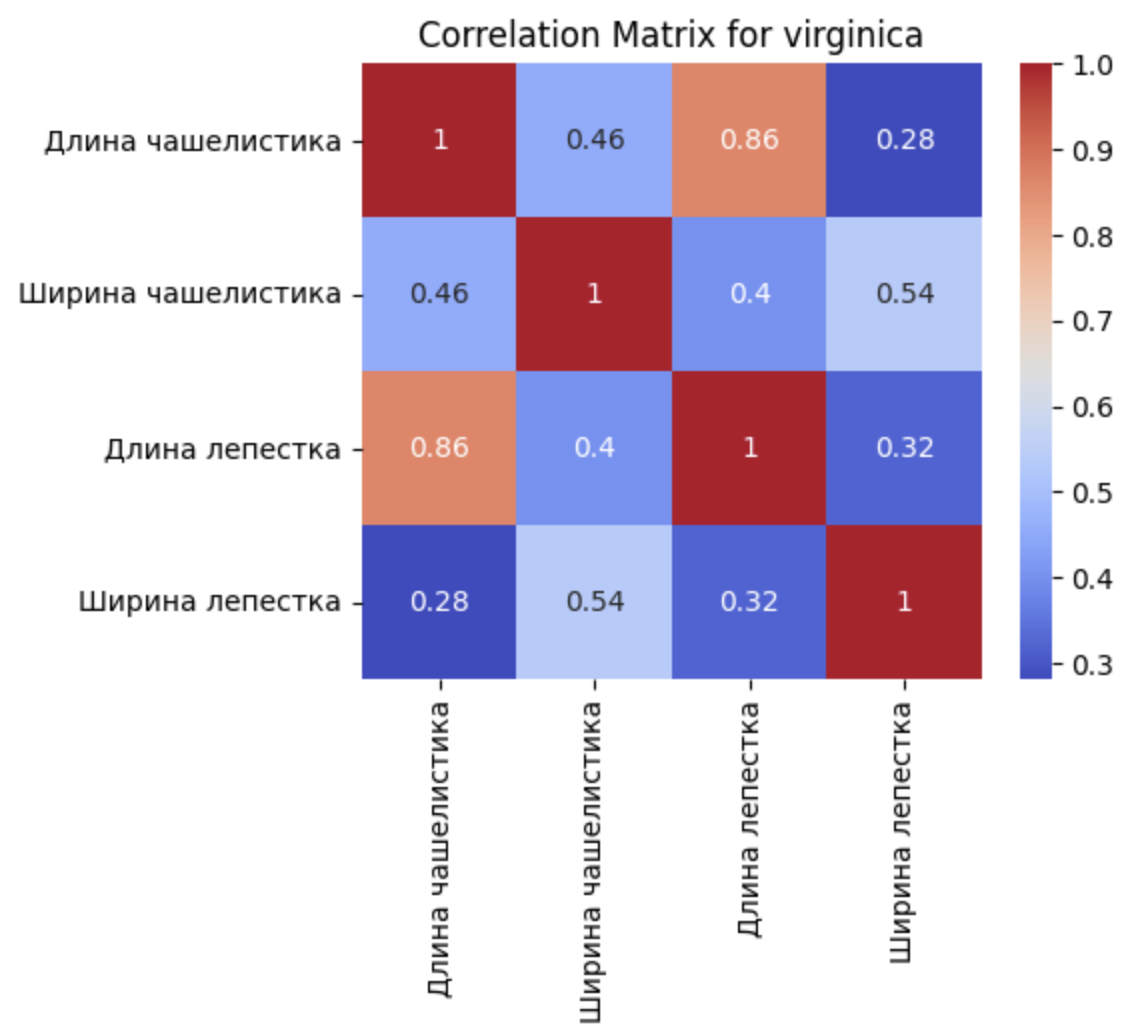
\includegraphics[width=\textwidth]{images/7.png}
	\end{center}
	\caption{Матрица корреляции признаков для класса <<virginica>>}
	\label{img:7}
\end{figure}

\section{Результат классификации}

\begin{lstlisting}[label=lst:2,caption=Отчёт по результатам классификации]
	Classification Report:
	precision    recall  f1-score   support
	
	setosa       			 1.00      1.00      1.00        12
	versicolor       	 0.94      0.94      0.94        16
	virginica       	 0.94      0.94      0.94        17
	
	accuracy                           		 0.96        45
	macro avg       	 0.96      0.96      0.96        45
	weighted avg       0.96      0.96      0.96        45
	
	Additional Metrics:
	MCC: 0.9326
\end{lstlisting}

\begin{figure}
	\begin{center}
		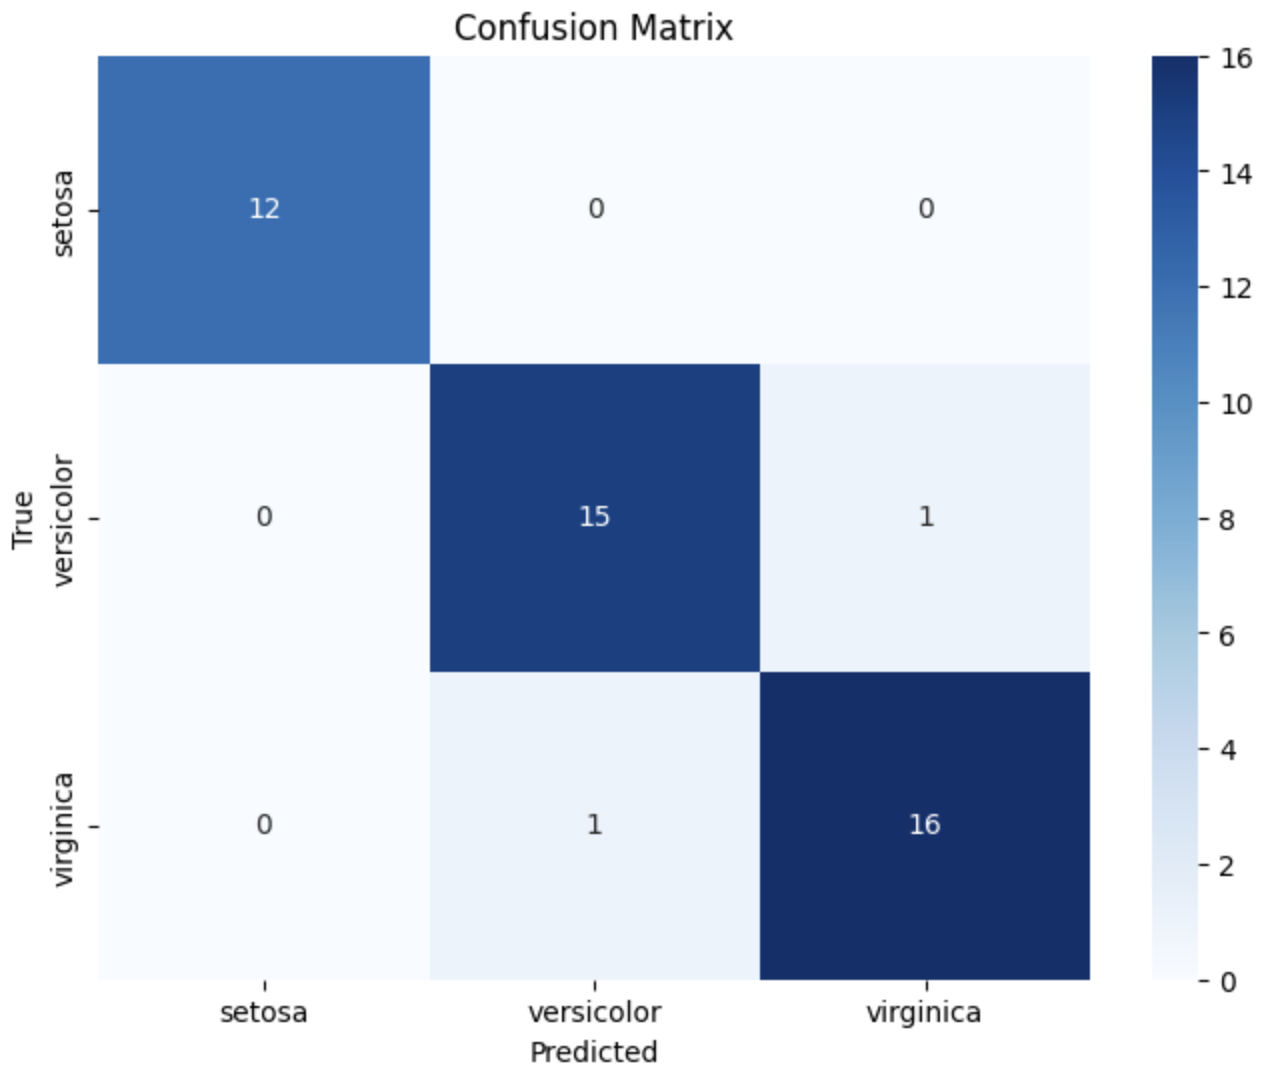
\includegraphics[width=\textwidth]{images/8.png}
	\end{center}
	\caption{Матрица ошибок}
	\label{img:8}
\end{figure}

\begin{figure}
	\begin{center}
		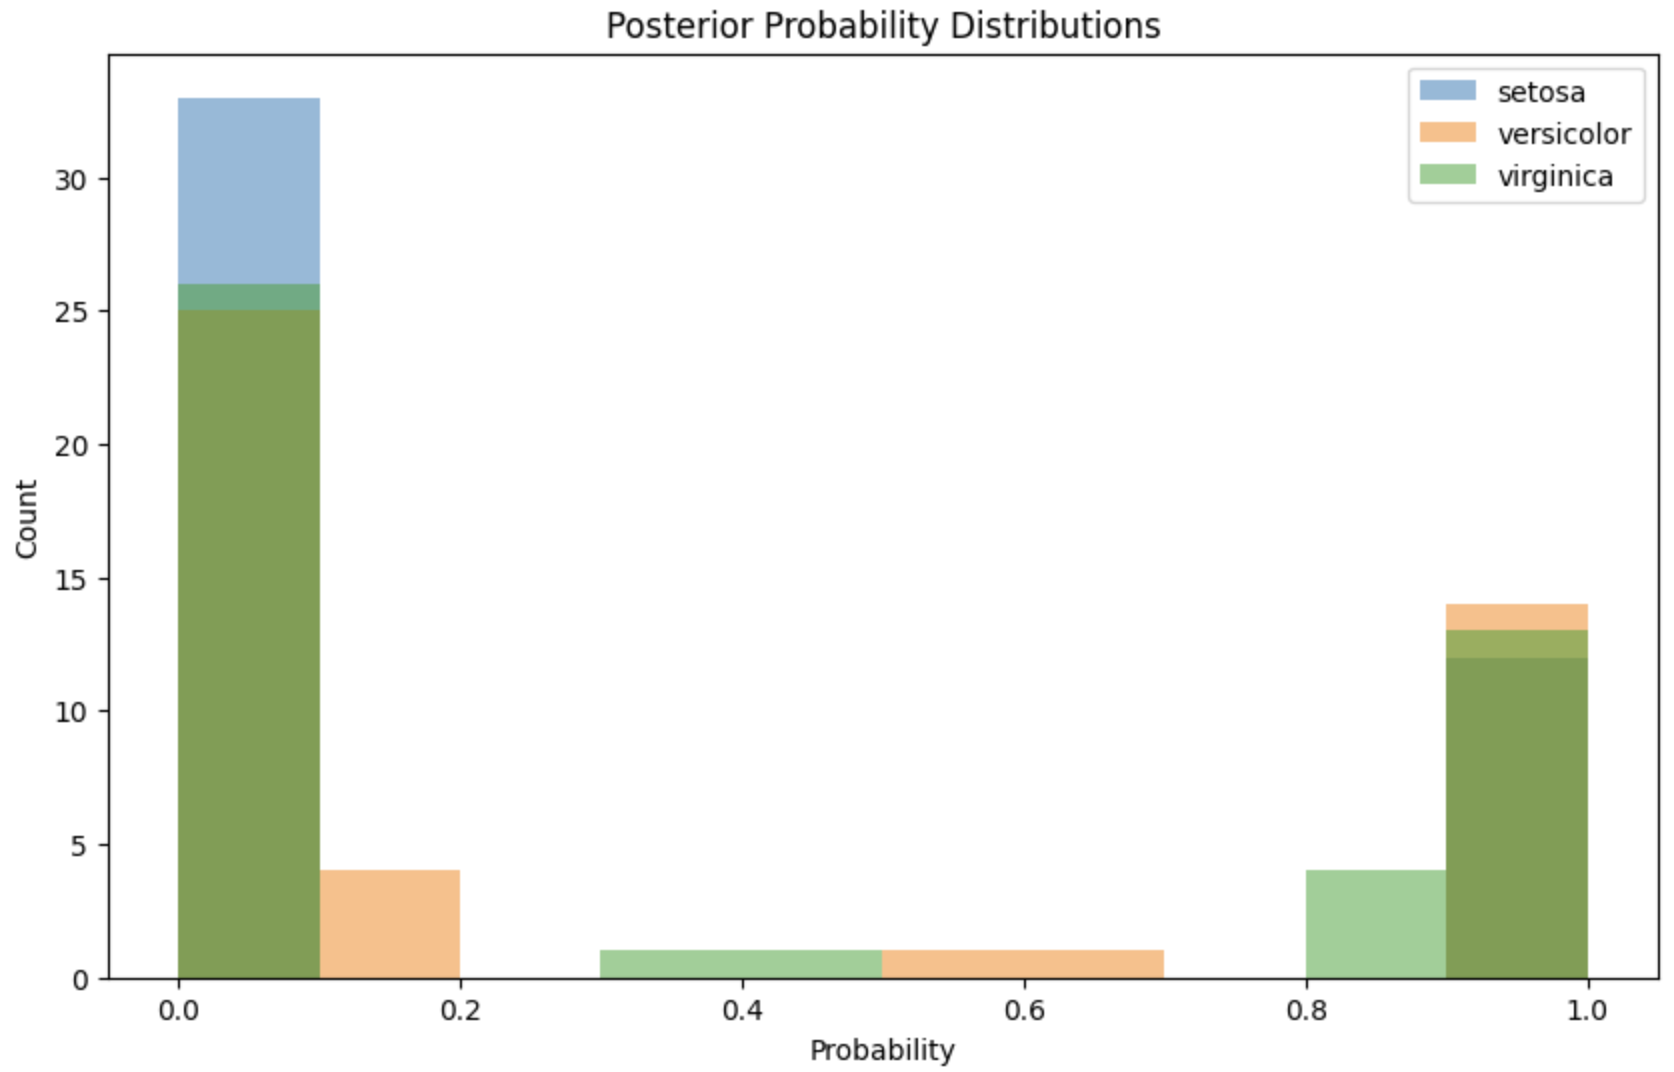
\includegraphics[width=\textwidth]{images/9.png}
	\end{center}
	\caption{Апостериорное распределение вероятностей для каждого класса}
	\label{img:9}
\end{figure}

\clearpage
